\documentclass[lettersize,journal]{IEEEtran}
\usepackage{amsmath,amsfonts}
\usepackage{algorithmic}
\usepackage{algorithm}
\usepackage{array}
\usepackage[caption=false,font=normalsize,labelfont=sf,textfont=sf]{subfig}
\usepackage{textcomp}
\usepackage{stfloats}
\usepackage{url}
\usepackage{verbatim}
\usepackage{graphicx}
\usepackage{cite}
\usepackage{longtable} % for tables
\usepackage{booktabs} % for tables

\hyphenation{op-tical net-works}
\setlength{\parindent}{0pt}

\begin{document}

\title{Neural Networks-Deep Learning \\ 3rd Assignment}
\author{Papadakis Konstantinos Fotios}
% The paper headers
\markboth{Neural Networks-Deep Learning, 3rd Assignment, 2024}
\maketitle

\begin{abstract}
This is the third Assignment of the course "Neural Networks-Deep Learning". It expands our 
knowledge on neural networks by creating an transformer neural network which is trained on 
the MNIST dataset. The network takes as input an image from the dataset and returns an image
depicting the next image in the sequence, as generated by the transformer itself.  
\end{abstract}

\section{Introduction}
\subsection{Dataset}
Reflecting on the higher complexity of the task at hand we have chosen to work with a simpler
dataset this time. The MNIST dataset is a collection of 70.000 images of handwritten digits,
each of which is $28x28$ pixels in size. The dataset is split in 60.000 training images and
10.000 test images. Here is a sample of the dataset:
\begin{figure}[H]   
    \centering
    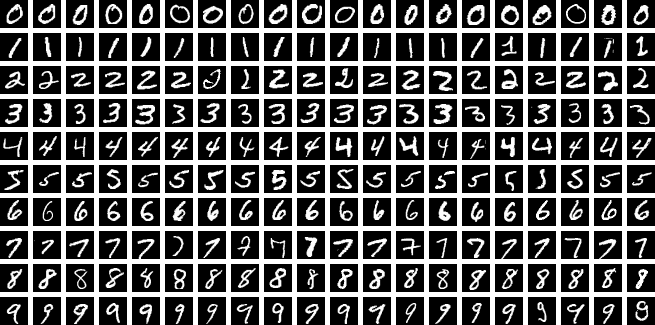
\includegraphics[width=0.5\textwidth]{MNIST_dataset_example.png}
    \caption{Sample of the MNIST dataset}
\end{figure}

\subsection{Transformers}
A transformer is a neural network architecture which is based on the multi-head attention
mechanism, where attention is a machine learning method that determines the importance of
each component relative to the the other components in a sequence. This architecture was 
first introduced in the paper "Attention is All You Need" by Vaswani et al. in 2017.

\smallskip

The transformer architecture is composed of an encoder and a decoder:
\begin{itemize}
    \item \textbf{Encoder}: 
    \item \textbf{Decoder}: 
\end{itemize}


\section{The Transformer Neural Network}
The approach we decided to follow revolves around a CNN encoder, a transformer and a CNN
decoder. Here are the specific roles of each component:
\begin{itemize}
    \item \textbf{Encoder}: The encoder extracts a latent representation of the input image.
    \item \textbf{Transformer}: The transformer modifies that representation to approximate 
    the next image in the sequence.
    \item \textbf{Decoder}: The decoder takes the modified representation and generates an
    image from it.
\end{itemize}

\subsection{Architecture}

\subsection{Results}

\vfill
\end{document}


